\chapter{Seguridad en el hogar}

% https://bricoladores.simonelectric.com/seguridad-en-el-hogar-que-debemos-proteger

% https://bricoladores.simonelectric.com/medidas-generales-basicas-de-seguridad-en-el-hogar

\section{Introducción}
La seguridad en el hogar es un tema relevante y delicado de manejar, principalmente cuando se trata del espacio vital más importante de todos, donde convive el ser humano. Sea del tipo que sea, en el hogar se establecen los vínculos más íntimos y personales; entonces la presencia de una persona en el hogar es un factor de seguridad de gran importancia. La mayoría de percances como intrusión de un extraño, allanamientos y robos se producen durante su ausencia. Los motivos para dejar un hogar vacío son varios: desde un viaje prolongado a salidas más o menos puntuales, regulares y/o diarias. Una vivienda vacía es más vulnerable que otra ocupada y este aspecto se toma en cuenta en el diseño de un sistema de seguridad para el hogar, el cual debe ofrecer características que ayuden a minimizar el impacto de las situaciones de peligro.\\

\section{Ausencia en el hogar}
En materia de seguridad del hogar, cualquier precaución, resulta de utilidad para prevenir, que ocurran incidentes y mantener protegidos a los seres más cercanos. De hecho el objetivo de la seguridad implica la toma de precauciones necesarias para que un lugar sea seguro para las personas.Incluso las personas más retraídas y amantes de la soledad y el aislamiento deben, en un momento u otro, salir de su residencia habitual, algo que se convierte en largas horas de ausencia en la mayoría de los casos (evidentemente por trabajo, obligaciones académicas y otros menesteres cotidianos), y ocasionalmente, con mayor o menor asiduidad, por otras razones menos frecuentes (viajes, vacaciones, etc).\\
 
Todas las posibles situaciones a presentarse se definen en función del tiempo de ausencia; de modo que se establecen distintos casos con aspectos peculiares y específicos referentes a la seguridad y los riesgos; por ejemplo exponer las medidas de protección más básicas y elementales que siempre deben tomarse en cuenta, como el contrato de un seguro para la vivienda (con elementos importantes que figuran en toda póliza para su elección y contratación).\\

Un seguro contra robos puede proteger de alguna manera los daños materiales que pueden ocurrir, pero incluso para probar la veracidad del suceso es necesario presentar pruebas visuales que sirvan de referencia en la denuncia. Una imágen como en la figura \ref{fig:intruso} puede ayudar incluso en una investigación.\\

\begin{figure}[H]
    \begin{center}
        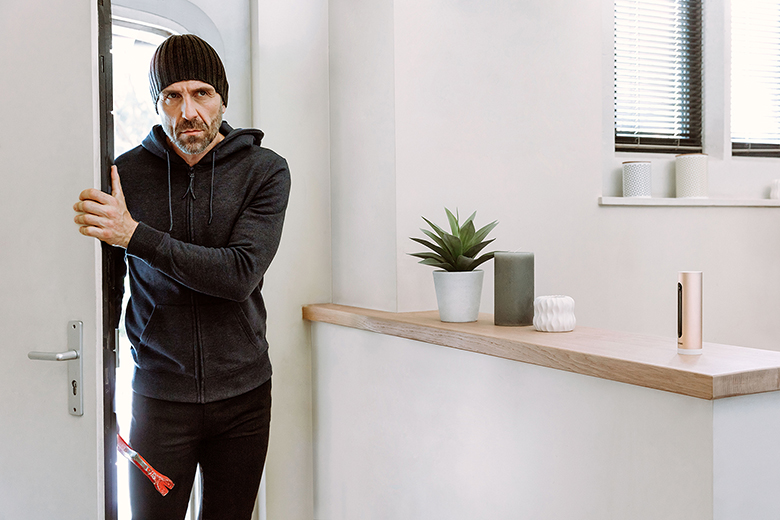
\includegraphics[width=7cm]{img/capitulo_3/intruso.jpg}
    \end{center}
    \begin{center}
        \caption{Ilustración ejemplo de un intruso.}
        Fuente: Web
        \label{fig:intruso}
    \end{center}
\end{figure}

A continuación se detallan las situaciones más comunes que pueden presentarse, con sus respectivas acciones sugeridas para disminuir el peligro.\\

\subsection{Ausencias cotidianas}
Las ausencias diarias de horas o minutos son las más comunes y brindan oportunidades a asaltantes atentos. Para este caso se puede tener en cuenta medidas de protección sencillas y sin complicaciones que cualquiera puede llevar a cabo apenas sin inversión alguna. Asegurar los cierres de los accesos a la vivienda, disimular las ausencias o evitar proporcionar información sobre nuestros hábitos son algunas de las medidas que se exponen para evitar intrusiones no deseadas en el hogar.\\
 
% Como situación perteneciente a este grupo de supuestos, pero con riesgos añadidos y particularidades propias que obligan a prestarle una atención especial, se tratará aparte el caso de ausencias puntuales dejando en la vivienda a niños, personas mayores o dependientes sin nadie a su cargo. Evidentemente, aquí se tratarán amenazas y riesgos internos de la vivienda, tales como manipulaciones indebidas de instalaciones y componentes de especial peligrosidad, o la atención a emergencias que puedan suceder durante ausencias breves.\\

\subsection{Ausencias de termino medio}
Cuando uno sale de casa previamente sabe si uno va ha volver al cabo de pocas horas, de unos días o de semanas; en cada caso se pueden presentar algunas peculiaridades y riesgos específicos que se deben afrontar de distintos modos. En este supuesto, tras las ausencias cotidianas, se detallan los casos de ausencias de pocos días, especialmente en fines de semana, puentes festivos y vacaciones cortas. En estas situaciones convergen la necesidad de contar con alarmas y avisadores técnicos, con la de disponer de sistemas de alarma y dispositivos antiintrusión los cuales, como veremos, pueden ser de muy diversa índole.\\

\subsection{Ausencias prolongadas}
Las vacaciones y las estancias de cierta duración en lugares alejados de nuestras residencias habituales ofrecen oportunidades únicas a posibles asaltantes. No ofrecer información sobre nuestro paradero, tratar de evitar el efecto de vivienda vacía, contar con la supervisión regular de alguien de confianza en nuestra ausencia y mantener a buen recaudo bienes u objetos de valor serán, en estos casos, las principales prioridades (sobre todo en el caso de las segundas residencias, una cuestión que también consideraremos detalladamente como caso diferenciado).\\

\section{Situaciones de riesgo}
\subsection{Presencia de instrusos}
Un intruso o persona ajena siempre representa un peligro en el interior de nuestro hogar y aún más cuando se desconoce el motivo de su presencia. La posibilidad de robos en cualquier cuidad del mundo esta presente y aun mas cuando este entra al interior de un hogar forzando cerraduras, encapuchado especialmente cuando los habitantes de la casa no estan. En la figura \ref{fig:ladron}, se muestra una ilustracion de ejemplo de un intruso forzando la puerta de una casa.\\

\begin{figure}[H]
    \begin{center}
        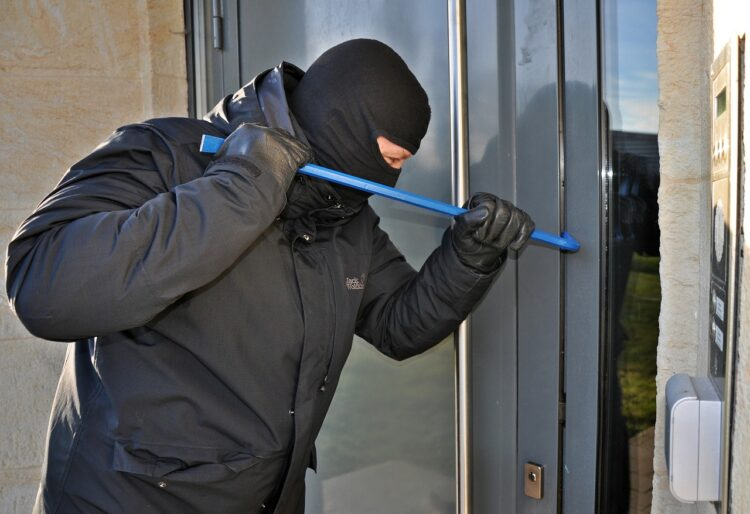
\includegraphics[width=5cm]{img/capitulo_3/burglar.jpg}
    \end{center}
    \begin{center}
        \caption{Ilustración ejemplo de un ladrón.} 
        Fuente: Web
        \label{fig:ladron}
    \end{center}
\end{figure}

\subsection{Fuego y humo}
El fuego es una reacción quimica, donde un conjunto de partículas o moléculas incandecentes en materia combustible es capaz de emitir calor y luz. Con el calor se pueden llegar a desintegrar muchos objetos y estos mismos servir de combustion para que el fuego se expanda.
Este fenómeno es uno de los principales causantes de tragedias en la actualidad, tanto como incendios forestales y/o colectivos, incendios en interiores, como ser casas, departamentos o sitios cerrados. En la figura \ref{fig:fuego} se visualiza la facilidad con la que el fuego puede expandirse en interiores.\\

\begin{figure}[H]
    \begin{center}
        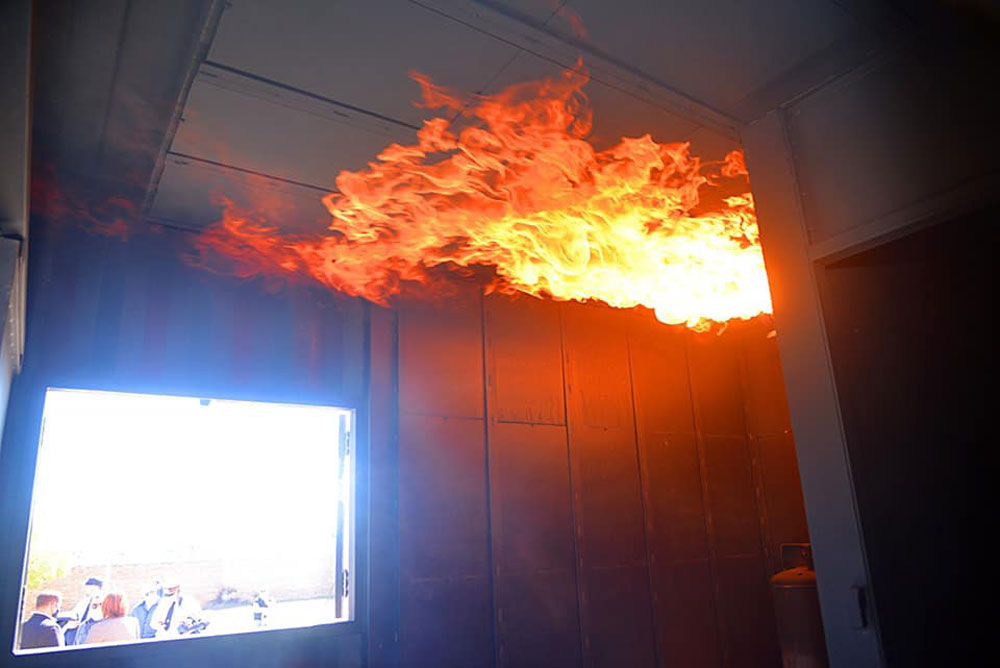
\includegraphics[width=5cm]{img/capitulo_3/fuego_en_interiores.jpg}
    \end{center}
    \begin{center}
        \caption{Ilustración ejemplo de fuego en interiores.} 
        Fuente: Web 
        \label{fig:fuego}
    \end{center}
\end{figure}

El humo acompañado del fuego son elementos muy perjudiciales tanto como a las personas como al medio ambiente en general. El humo es uno de los factores principales que afectan a la salud respiratoria de las personas y animales en general. Identificar a tiempo la presencia de humo puede incluso prevenir y/o predecir la organización de fuego  evitar tragedias.\\

En la figura \ref{fig:humo}, se visualiza como la presencia de humo puede ayduar a alertar de que hay fuego en el interior de una casa o habitación.\\

\begin{figure}[H]
    \begin{center}
        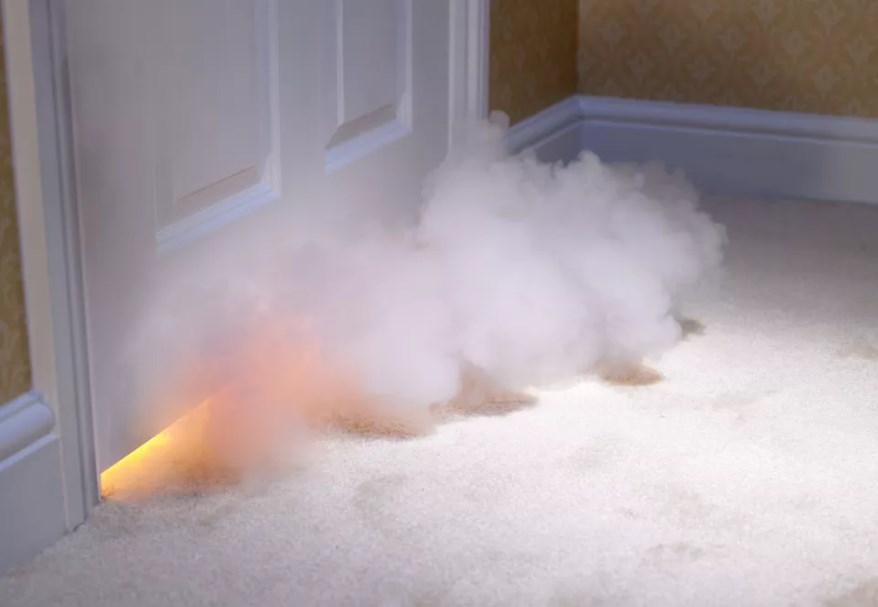
\includegraphics[width=5cm]{img/capitulo_3/fuego_en_el_cuarto.jpg}
    \end{center}
    \begin{center}
        \caption{Ilustración de la presencia de fuego y humo en una habitación cerrada.}
        Fuente: Web.
        \label{fig:humo}
    \end{center}
\end{figure}

\section{Sistemas de seguridad}
En el mercado, existe una gran variedad de artefactos, que están al alcance de todos para proteger los hogares frente a cualquier tipo de amenaza, tanto interna como externa. Los más eficaces y eficientes, son los sistemas electrónicos de seguridad. No obstante, sea cual sea la opción elegida se debe tener en cuenta los siguientes riesgos y amenazas:\\

\begin{itemize}
    \item \textbf{Allanamientos, intrusiones y vandalismo:} riesgos procedentes del exterior, que se pueden mitigar fácilmente instalando cierres de alta seguridad en los accesos a la vivienda, alarmas antiintrusión u otros mecanismos disuasorios.
    \item \textbf{Accidentes domésticos:} riesgos procedentes del interior de hogar que pueden poner en riesgo la integridad física y/o moral de sus habitantes, tanto personas como mascotas, así como los bienes que contienen e incluso la misma infraestructura.
\end{itemize}

Las alarmas técnicas (alertas de fugas y escapes) y de emergencia son los sistemas más adecuados para proteger una vivienda. También es preciso tomar las medidas oportunas para proteger los componentes más sensibles del hogar (instalaciones de suministros y otros elementos de riesgo) de manipulaciones indebidas, golpes y otro tipo de percances que pueden ocasionar accidentes o situaciones indeseables.\\

\subsection{Alarmas}

Las alarmas son artefactos sonoros que emiten un sonido que provoca la alerta en las personas. Existen de diferentes tipos, medidas y campo de uso. El volúmen y el sonido es claramente diferenciado de cualquier objeto que emita un sonido cualquiera. Este objeto es utilizado generalmente para poner en alerta a todas las personas que lleguen a escucharlo y/o comunicar peligro.
En la figura \ref{fig:bocinas} se puede apreciar un modelo particular de alarmas sonoras.

\begin{figure}[H]
    \begin{center}
        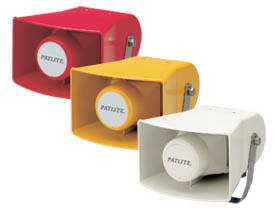
\includegraphics[width=3cm]{img/capitulo_3/alarmas.jpg}
    \end{center}
    \begin{center}
        \caption{Ilustración de alarmas con sonido.}
        Fuente: Web.
        \label{fig:bocinas}
    \end{center}
\end{figure}

\subsection{Sensores}
Los sensores son dispositivos que captan magnitudes físicas (variaciones de luz, temperatura, sonido, etc.) u otras alteraciones de su entorno. Los detectores de humo son dispositivos desarrollados para detectar la presencia de un incendio en el interior de un edificio. En la figura \ref{fig:detector_humo} se aprecia un modelo en particular de sensor de detección de humo.\\

\begin{figure}[H]
    \begin{center}
        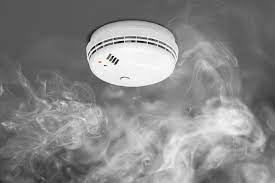
\includegraphics[width=5cm]{img/capitulo_3/sensor_de_humo.jpg}
    \end{center}
    \begin{center}
        \caption{Ilustración de detector de humo.}
        Fuente: Web.
        \label{fig:detector_humo}
    \end{center}
\end{figure}

\subsection{Cámaras}

Las cámaras son dispositivos que permiten registrar imágenes estáticas y en movimiento. Específicamente las cámaras de vigilancia son las que se encargan de grabar todo lo que puede ocurrir en una casa o negocio. Contar con este tipo de cámara puede proporcionar sensación de seguridad y protección. Disponer de este tipo de sistemas puede resultar ser una solución para mantenerse protegido. El desarrollo de la tecnología ha logrado que el sector de la seguridad disponga de equipos eficientes y con diversas funcionalidades. En la figura \ref{fig:camaras} se visualizan diferentes modelos de cámaras de seguridad que se encuentran en el mercado.\\

\begin{figure}[H]
    \begin{center}
        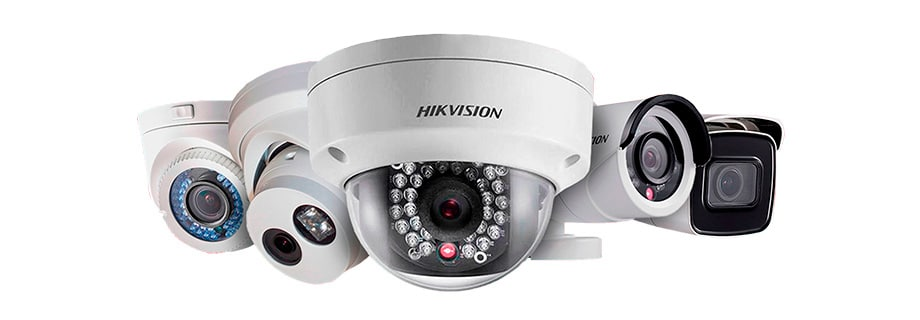
\includegraphics[width=6cm]{img/capitulo_3/camaras.jpg}
    \end{center}
    \begin{center}
        \caption{Ilustración de diversas cámaras de seguridad.}
        Fuente: Web.
        \label{fig:camaras}
    \end{center}
\end{figure}

El tipo más común en el mercado son las cámaras de interiores ya que son las más sencillas y económicas del mercado ya que no necesitan mucho mecanismo ni protección. En la figura \ref{fig:camara} se visualiza un ejemplo de cámara de interiores.\\

\begin{figure}[H]
    \begin{center}
        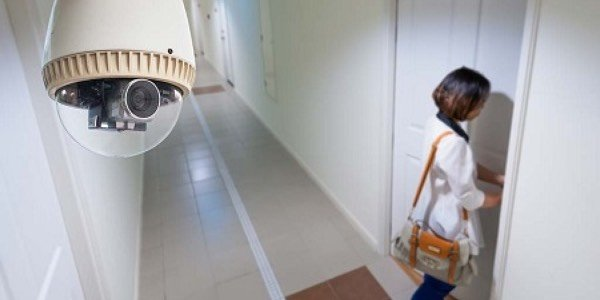
\includegraphics[width=5cm]{img/capitulo_3/camara_de_interiores.jpg}
    \end{center}
    \begin{center}
        \caption{Cámara de vigilancia de interiores.}
        Fuente: Web.
        \label{fig:camara}
    \end{center}
\end{figure}

Seguridad y vigilancia son aspectos que se requieren en todo el mundo; gobiernos, empresas, instituciones financieras, organizaciones de salud, necesitan cierto grado de medidas de seguridad y como resultado se generó un dramático incremento en la demanda de aplicaciones de seguridad como por ejemplo video vigilancia, monitoreo y grabación de: fronteras, puertos, transporte, hogares, corporaciones, instituciones educativas, lugares públicos, edificios, etc.\\

% Sistemas de videovigilancia inteligente La técnica clave del reconocimiento de la accion humana basada en la vision  por compoutadora consiste en describir y comprender los comportamientos humanos por medio de la vision por computadora.\\

% Este proceso es una tarea complicada e integra algunos campos de investigacion que incluyen el procesamiento de imagen, aperndizaje automatico, reconocimiento de patrones, etc.\\

% La detección de un objeto móvil consiste en separar las áreas de cambio en el video es decir en las imádgenes de fondo que comprenden el video, dicho de otra manera, separar correctamente las áreas y contornos del objetico movil. Es critico para el siguiente procesamiento la segementación efectiva \\
